% !TeX root = ../main.tex

\chapter{编译过程展示系统}

\section{展示系统设计与实现}

既然采用了 Nanopass 策略来实现编译器,
在编译的过程中输出每一趟编译过程的结果是很自然的想法。
我们可以通过观察每一个编译过程的输入和输出来确保我们的想法是可行的,我们的实现是正确的。
但是,在终端中从上到下打印出的编译结果不方便进行对比,也缺乏交互性。

因此,本文实现了一个图形界面程序,
允许我们在一个能自动格式化Lisp源码的文本框中输入源程序,
然后在一系列文本框中展示编译过程的每一趟的转换结果,
并在指定目录中生成最终的汇编代码和可执行文件。

本文采用了Racket的framework库图形用户接口来实现展示系统,
该库是对Racket的原生图形用户接口 racket/gui 库的二次封装,
提供了许多更易用的类和函数。
本文使用 \code{racket:text\%} 类的实例作为源程序的输入框,
该输入框能自动缩进Lisp类语言的源代码,高亮所有Racket关键字。
展示中间结果的文本框同样使用该类,但对它们调用 lock 函数进行锁定,
这样这些文本框就会停止高亮并且无法被编辑。由于中间过程数量众多,
这样做可以减少程序运行时的开销,同时也防止由于误操作导致中间结果被修改。

\section{展示系统运行效果}

图\ref{fig:gui-init}展示了在该编译过程展示系统中输入一段源程序的效果。
\begin{figure}[h]
\centering
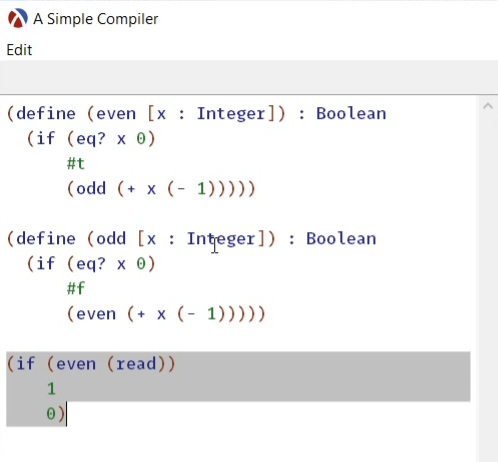
\includegraphics[width=0.52\textwidth]{figures/gui-init2.png}
\caption{展示系统输入源程序}
\label{fig:gui-init}
\end{figure}

点击编译按钮后,
所有的编译过程的中间结果以及最后的x86-64代码都将并排展示在一系列横向排列的文本框中,
方便我们对各个中间结果进行横向对比,
指定的目录下也会生成最终的可执行文件。
展示系统还利用graphviz软件绘制了所有函数的干涉图,
这些图片也会以svg格式的文件存放在同一个目录下。
图\ref{fig:gui-compile}展示了点击编译按钮后的展示系统。
图\ref{fig:gui-interf-graph}展示了
图\ref{fig:gui-init}中的\code{even}函数的变量和寄存器干涉图。

\begin{figure}[h]
\centering
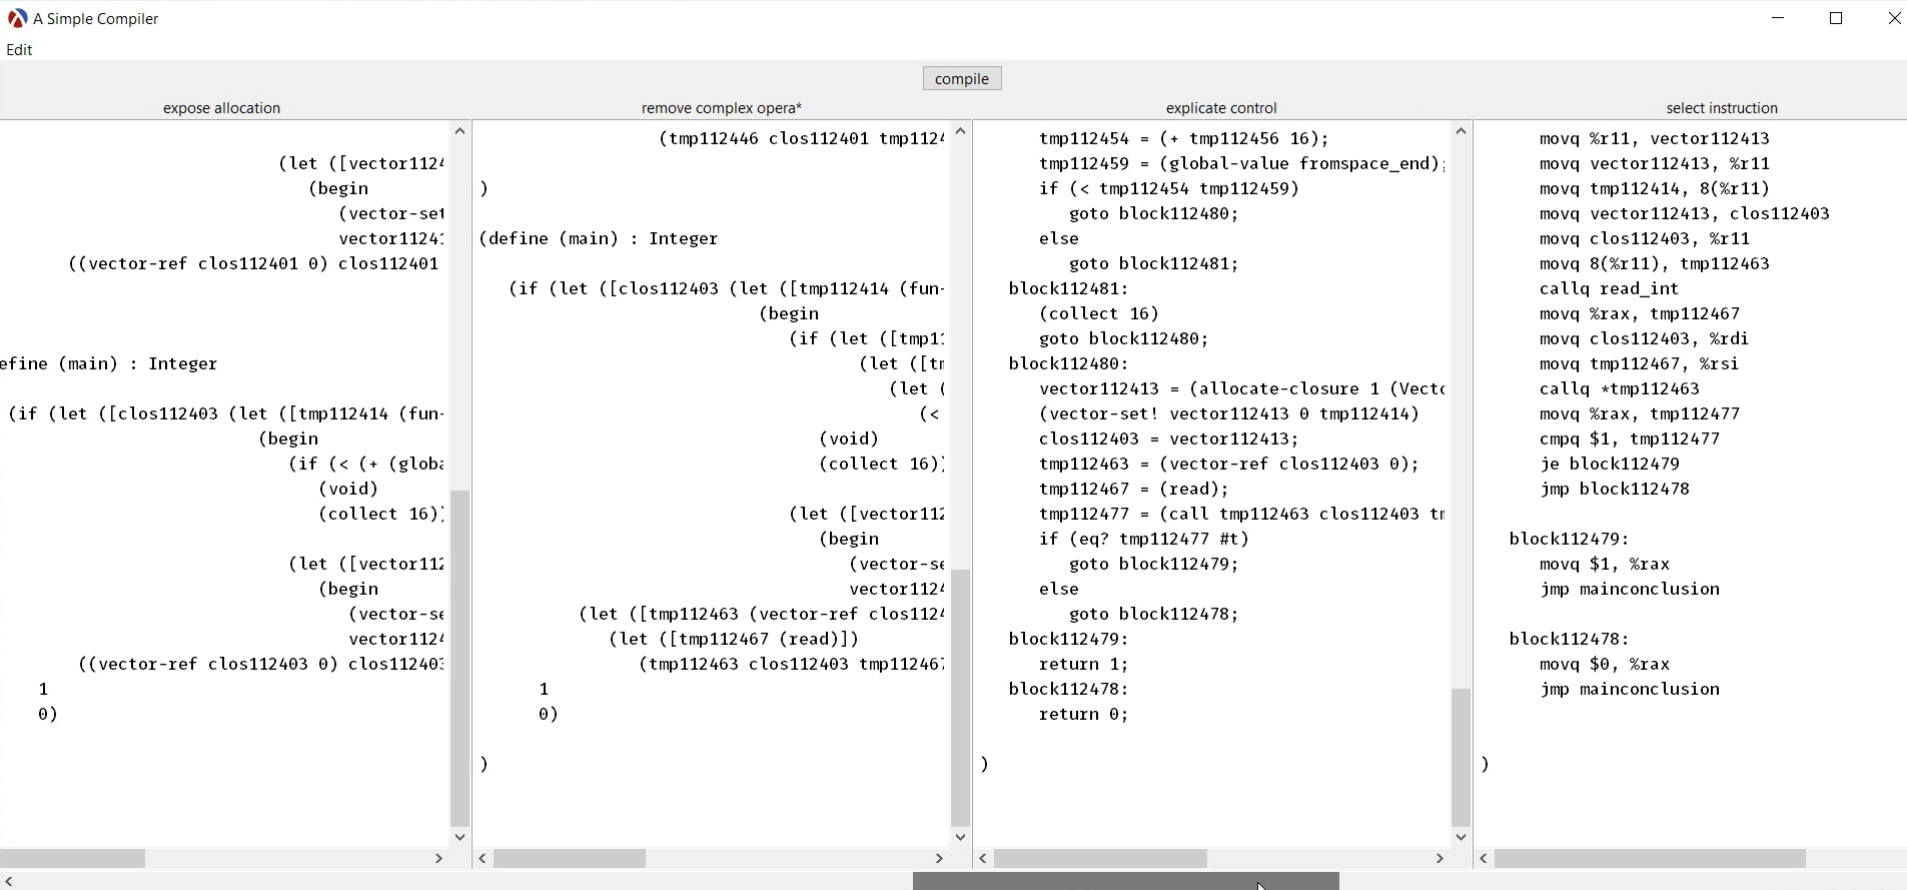
\includegraphics[width=\textwidth]{figures/gui-compile.png}
\caption{并列展示编译过程的中间结果}
\label{fig:gui-compile}
\end{figure}

\begin{figure}[h]
\centering
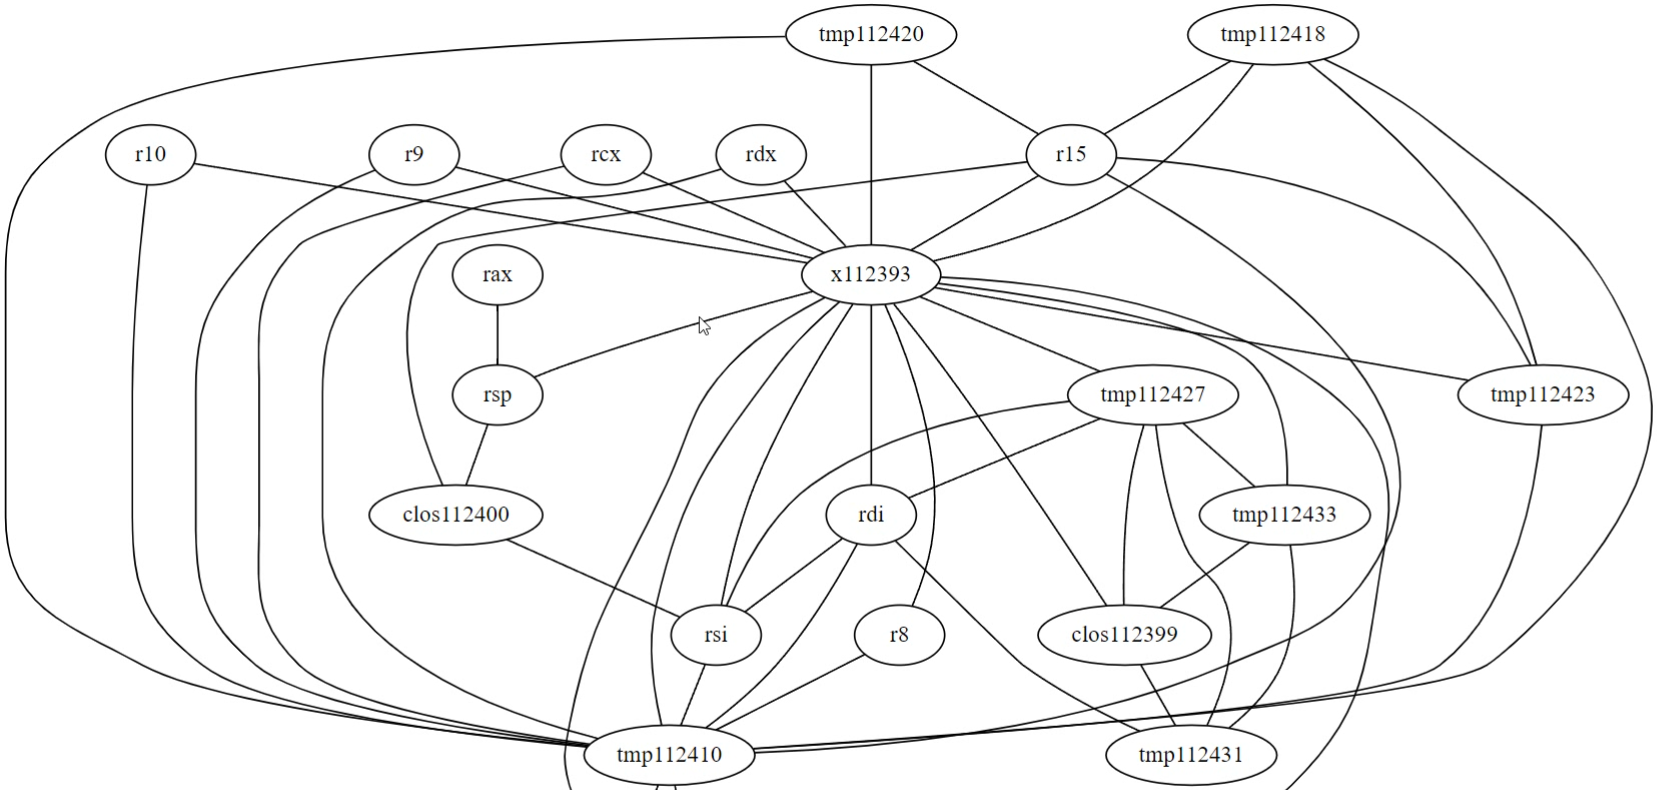
\includegraphics[width=\textwidth]{figures/gui-interf-graph.png}
\caption{调用graphviz绘制干涉图}
\label{fig:gui-interf-graph}
\end{figure}

最后,图\ref{fig:gui-result}展示了图\ref{fig:gui-init}中示例程序的运行结果。

\begin{figure}[h]
\centering
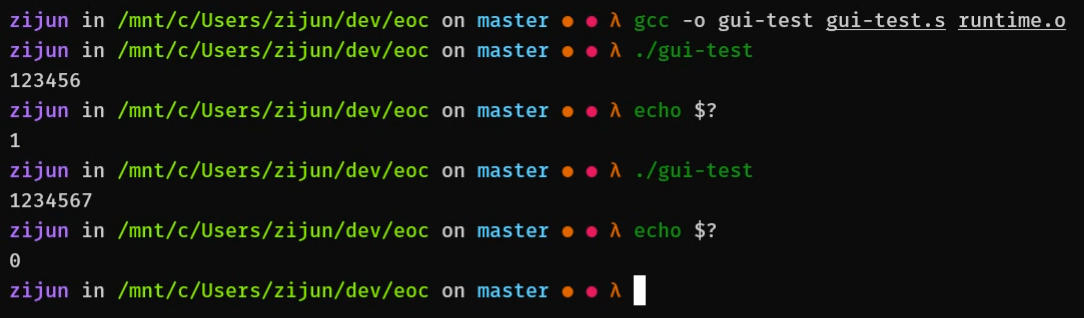
\includegraphics[width=\textwidth]{figures/gui-result.png}
\caption{示例程序的运行结果}
\label{fig:gui-result}
\end{figure}


\section{本章小结}

本章首先说明了对于 Nanopass 策略的编译器而言,
设计一个交互式的编译过程展示系统的意义和必要性,
然后简要介绍了本文的实现方法,最后展示了系统的具体效果。
